\documentclass[a4paper,12pt]{report}

\usepackage[dutch]{babel}           % Nederlands
\usepackage[latin1]{inputenc}       % speciale karakters

\usepackage{palatino} % font
\usepackage{graphicx} % figuren
\usepackage{float}
%\graphicspath{{}}
\usepackage{subcaption}

\usepackage[hyperfootnotes=false]{hyperref} % PDF bookmarks
\usepackage{titlesec}	
\usepackage{fancyhdr}

\renewenvironment{quote}                            % kleinere citaten
               {\list{}{\rightmargin\leftmargin}    %
                \item[]\small}                      %
               {\endlist}                           %

\setlength{\parindent}{0pt}         % indenteringen met witlijn
\setlength{\parskip}{1em}           %

\setlength{\hoffset}{-1cm}          % kleinere marges
\addtolength{\textwidth}{2cm}
\setlength{\voffset}{-1cm}
\addtolength{\textheight}{2cm}

\makeatletter                               % een witlijn tussen
\renewcommand{\footnoterule}{               % voetnoten en tekst
  \vspace{1em}                              %
  \kern-3\p@\hrule\@width.4\columnwidth     %
  \kern2.6\p@}                              %
\makeatother                                %
                                            %
                               
\usepackage[stable]{footmisc}               % pakket voor bep. voetnoten. (voetnoten in titels)

\usepackage{graphicx}   %afbeeldingen

\newcommand{\nroman}{\renewcommand{\thepage}{\roman{page}}\setcounter{page}{0}}     % romeinse nummers
\newcommand{\narabic}{\renewcommand{\thepage}{\arabic{page}}\setcounter{page}{1}}   % arabische nummers


%\bibliographystyle{plain}
%\usepackage[nottoc,section]{tocbibind}     % bibliografie in TOC, sectiegrootte
\setcounter{tocdepth}{3}                   % diepte van de TOC

\usepackage[linesnumbered,ruled,vlined]{algorithm2e} 		% Algoritmen
\usepackage{algpseudocode}
\renewcommand*{\listalgorithmcfname}{Lijst van algoritmen}	%
\renewcommand*{\algorithmcfname}{Algoritme}					%
\renewcommand*{\algorithmautorefname}{algoritme}	

\lhead{Brent Van Wynsberge}
\rhead{Project Algoritmen en Datastructuren III}



%%% TITEL EN AUTEUR %%%

\renewcommand{\title}{%
			Huffman compressie \\
			\large Project Algoritmen en Datastructuren III}
\renewcommand{\author}{
\textbf{\large Brent Van Wynsberge} \\
\small 3$^e$ bachelor Informatica, Universiteit Gent \\
\small Algoritmen en Datastructuren III \\
\small Stamnummer: 01201853 \\
}

%%% / / / %%%

\renewcommand{\maketitle}{
\thispagestyle{empty}
\begin{minipage}{3.5in}

\includegraphics{ugent.png}
\end{minipage}
\hfill
\begin{minipage}{3in}
\begin{flushright}
\author
\bigskip
\textbf{\today}
\end{flushright}
\end{minipage}
\vspace{5em}
\vspace*{\fill}
\begin{center}
\Huge{\title}
\end{center}
\vspace*{\fill}}

\titleformat{\chapter}{\normalfont\huge}{\thechapter.}{20pt}{\huge} %chapterformat
\newcommand{\bigO}[1]{$\bm{\mathcal{O}(#1)}$} %big O notatie
\usepackage{bm}

\begin{document}
\global\emergencystretch = .3\hsize

%%% INLEIDEND %%%
\nroman
\maketitle
\newpage

\tableofcontents
\newpage

\pagestyle{fancy}

%%% HOOFDSTUKKEN %%%
%%%%%%%%%%%%%\input{algemeen}
\newpage
\narabic

\chapter{Algoritmen}
In dit onderdeel bekijken we de pseudocode van alle ge\"implementeerde algoritmen. Wanneer er een niet triviale operatie opgeroepen wordt, wordt deze beschreven in het onderdeel 'Algemene Operaties'.\\ \\
De \Call{write}{foo} operatie heeft als betekenis: schrijf foo weg naar stdout. De operatie abstraheert het eventuele gebruik van buffers of de alignering van de bits weg. \\ \\
De \Call{read}{} operatie heeft als betekenis: lees de volgende byte van stdin. Analoog met \Call{write}{} abstraheert dit het gebruik van buffers weg en doet dit alsof de tekst altijd byte per byte wordt ingelezen.
%%%%Static
\section{Statische huffman}
\subsection{Algemene operaties}

\begin{algorithm}[H]
\caption{incrementWeight}
\SetAlgoLined	
\DontPrintSemicolon
$input$
}\;
\end{algorithm}

\begin{algorithm}[H]
\caption{readInput}
\SetAlgoLined	
\DontPrintSemicolon
\While{$(byte \gets$\Call{read}{ }$) \neq$ \textbf{EOF}}{
	$input.content[input.size\texttt{++}] \gets byte$\;
	\Call{incrementWeight}{input, byte}
}\;
\end{algorithm}

\subsection{Encoderen}

\begin{algorithm}[H]
\caption{encode}
\SetAlgoLined	
\DontPrintSemicolon
$input \gets$\Call{readInput}{ }\;	
$tree, max \gets$\Call{buildTree}{input}\;
$codes \gets$\Call{buildDictionary}{tree, max}\;
\Call{printTree}{tree}\;
\Call{encodeInput}{input, tree}\;
$zeros \gets 0$\;
\While{\textbf{not} \Call{full}{last\_byte}}{
	$last\_byte[current\_bit\texttt{++}] \gets 0$\;
	$zeros++$\;
}\;
\Call{write}{last\_byte}\;
\Call{write}{zeros}\;
\end{algorithm}

\subsection{Decoderen}

%%%%Adaptive
\section{Adaptive huffman}
\subsection{Algemene operaties}

\subsection{Encoderen}

\subsection{Decoderen}

%%%%%Sliding
\section{Adaptive huffman met sliding window}
\subsection{Algemene operaties}

\subsection{Encoderen}

\subsection{Decoderen}


%%%%%2p
\section{Two pass adaptive huffman}
\subsection{Algemene operaties}

\subsection{Encoderen}

\subsection{Decoderen}


%%%%%%Block
\section{Bloksgewijze adaptive huffman}
\subsection{Algemene operaties}

\subsection{Encoderen}

\subsection{Decoderen}


\chapter{Datasets}

\chapter{Experimenten}

%\begin{figure}[h]
%	\begin{subfigure}{\linewidth}
%		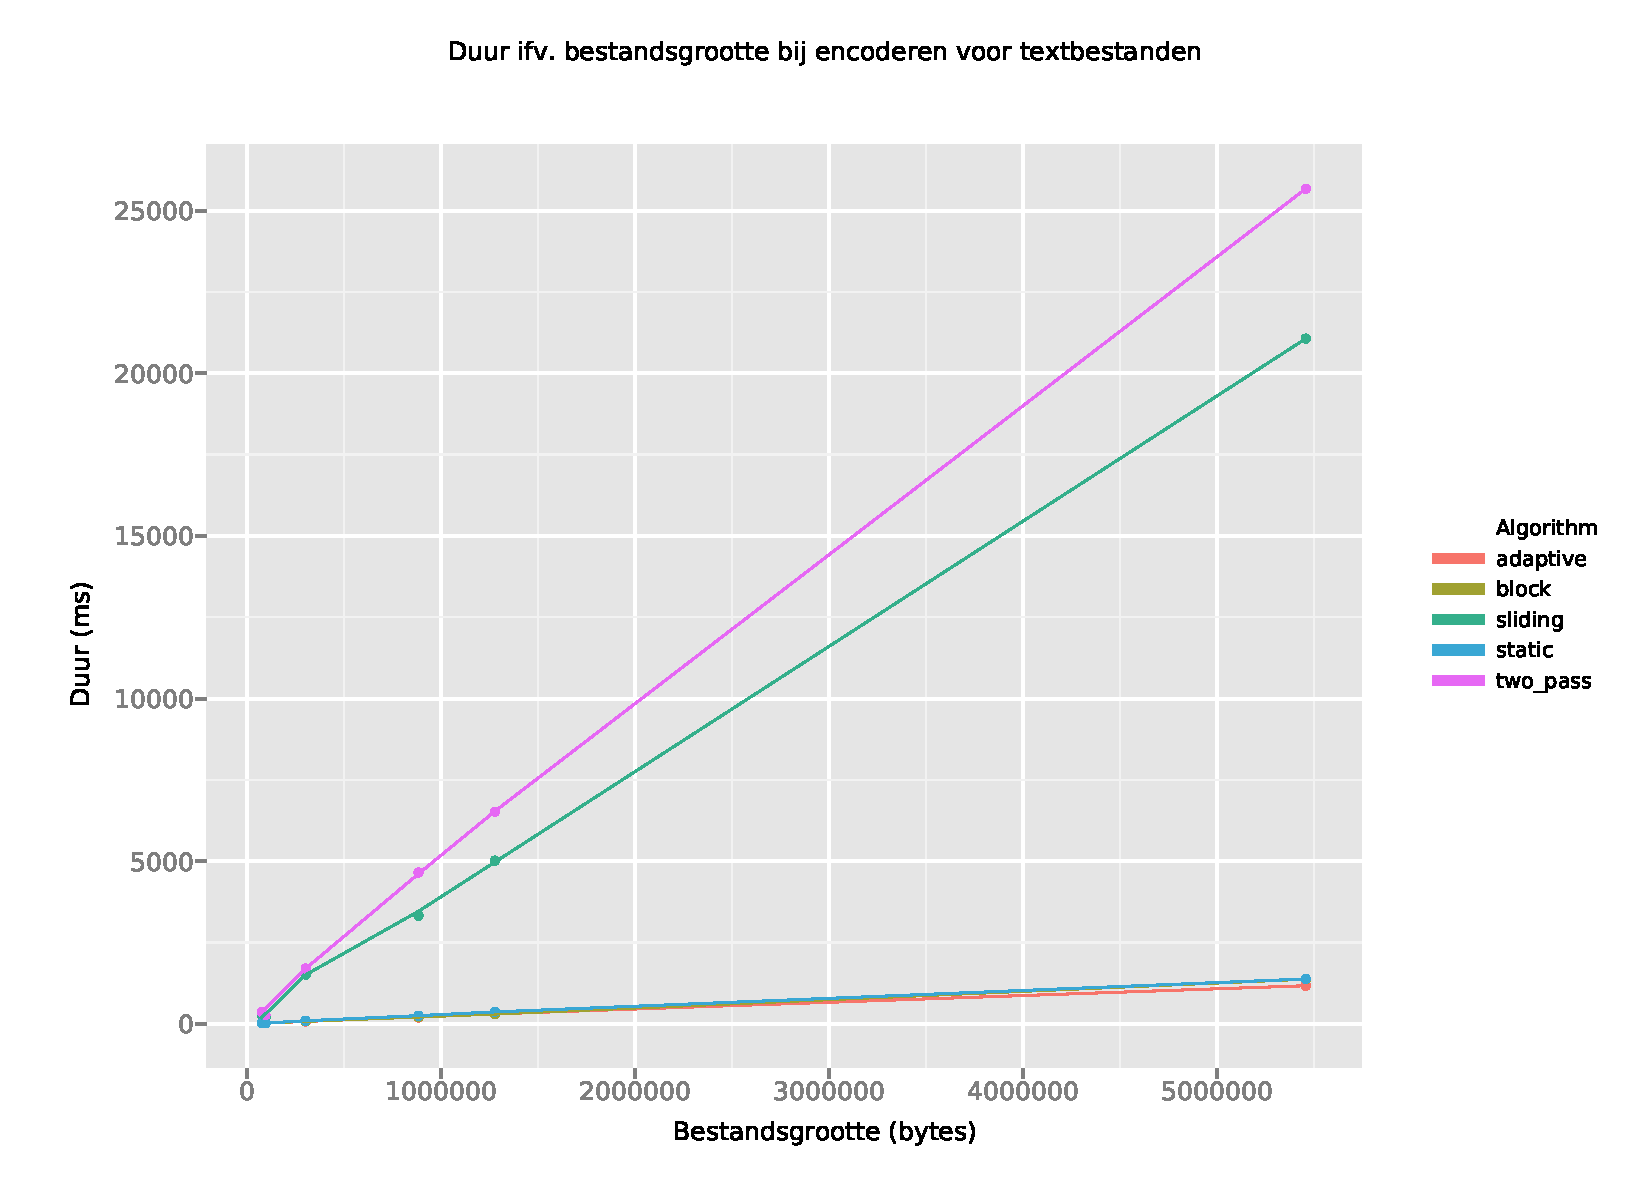
\includegraphics[width=.5\linewidth]{../experimenten/grafieken/duur/encode_textbestanden.pdf}\hfil
%		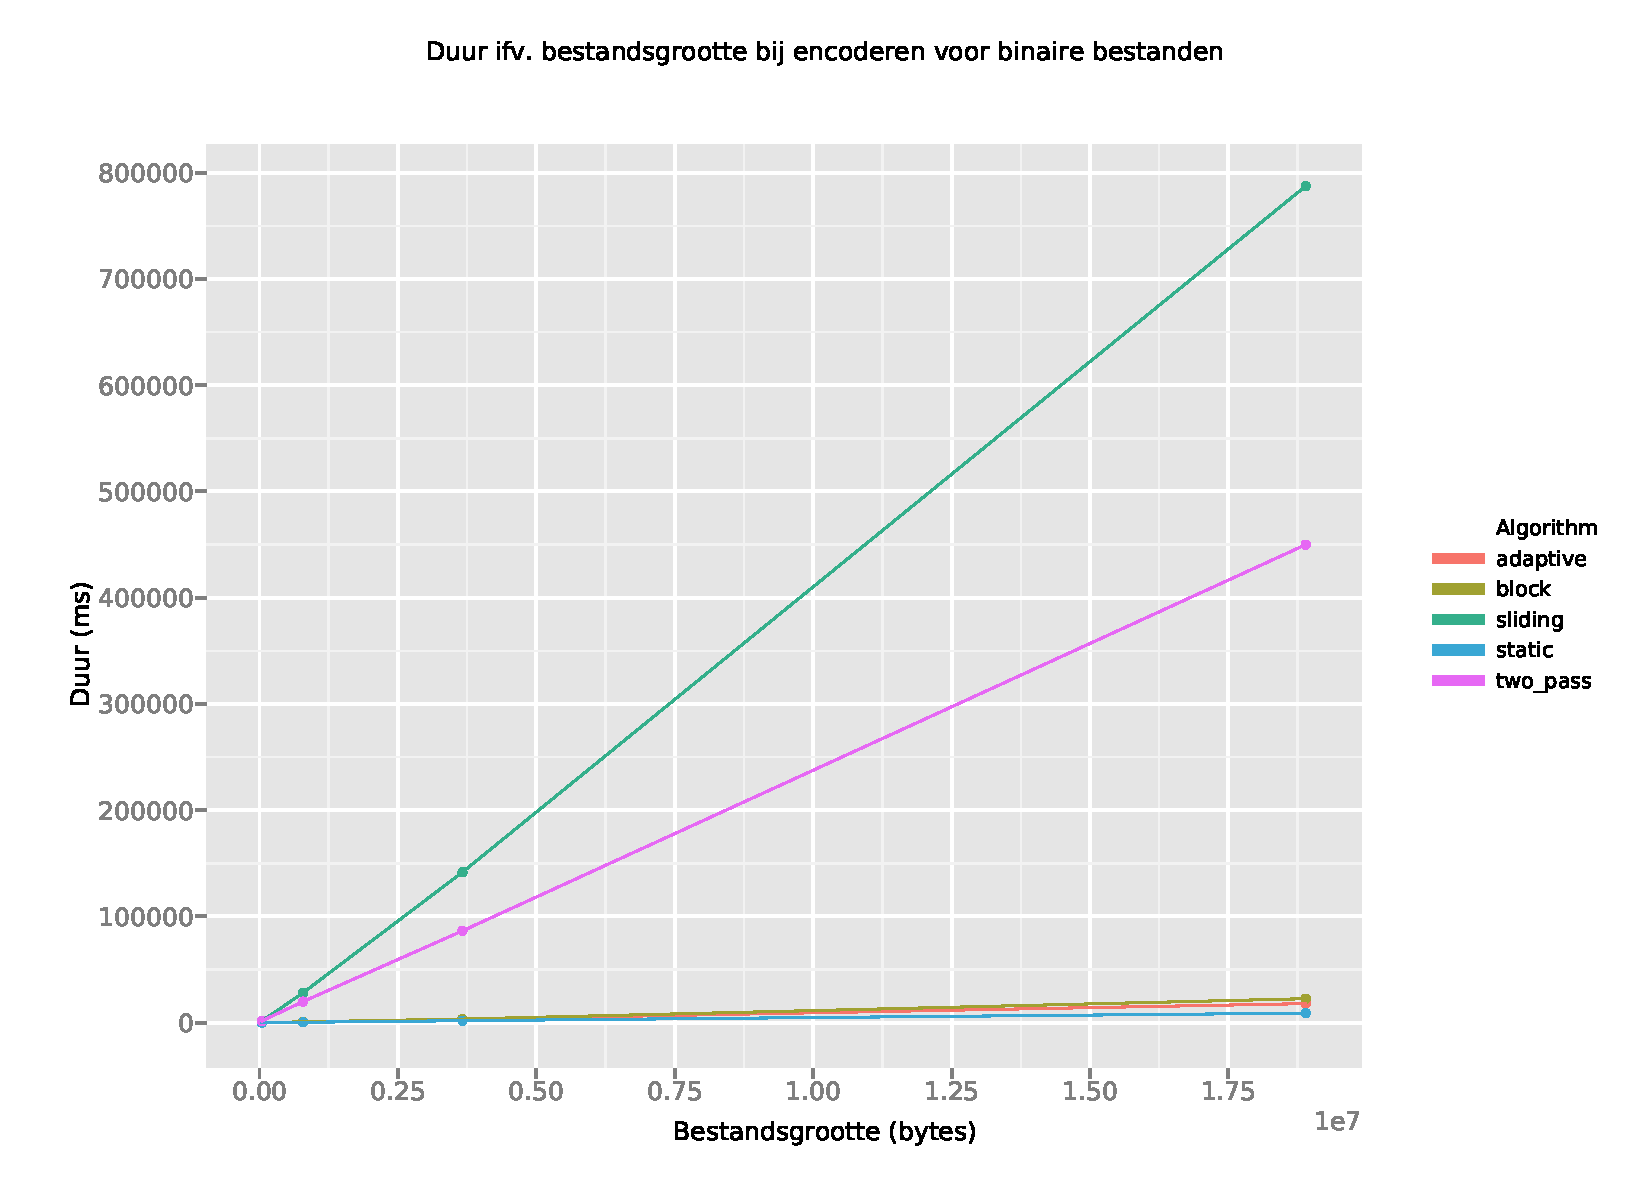
\includegraphics[width=.5\linewidth]{../experimenten/grafieken/duur/encode_binaire_bestanden.pdf}
%	\end{subfigure}
%	\begin{subfigure}{\linewidth}
%		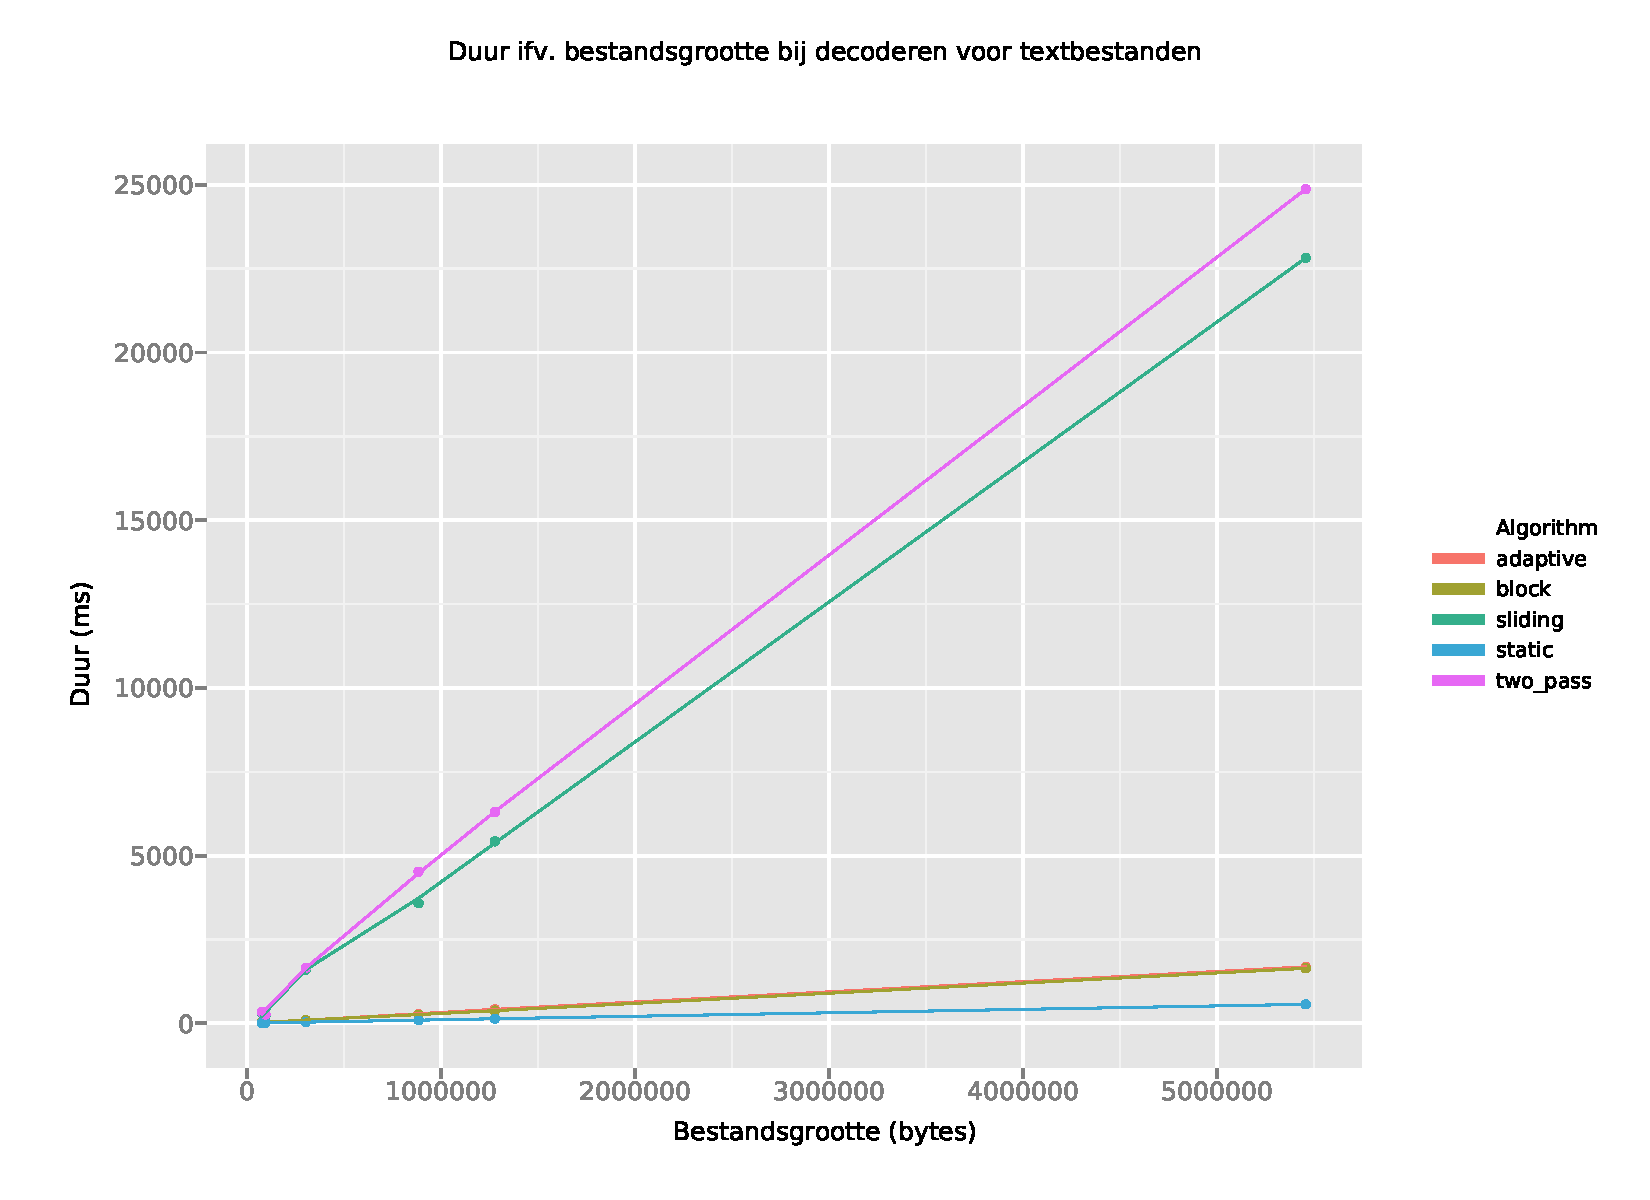
\includegraphics[width=.5\linewidth]{../experimenten/grafieken/duur/decode_textbestanden.pdf}\hfil
%		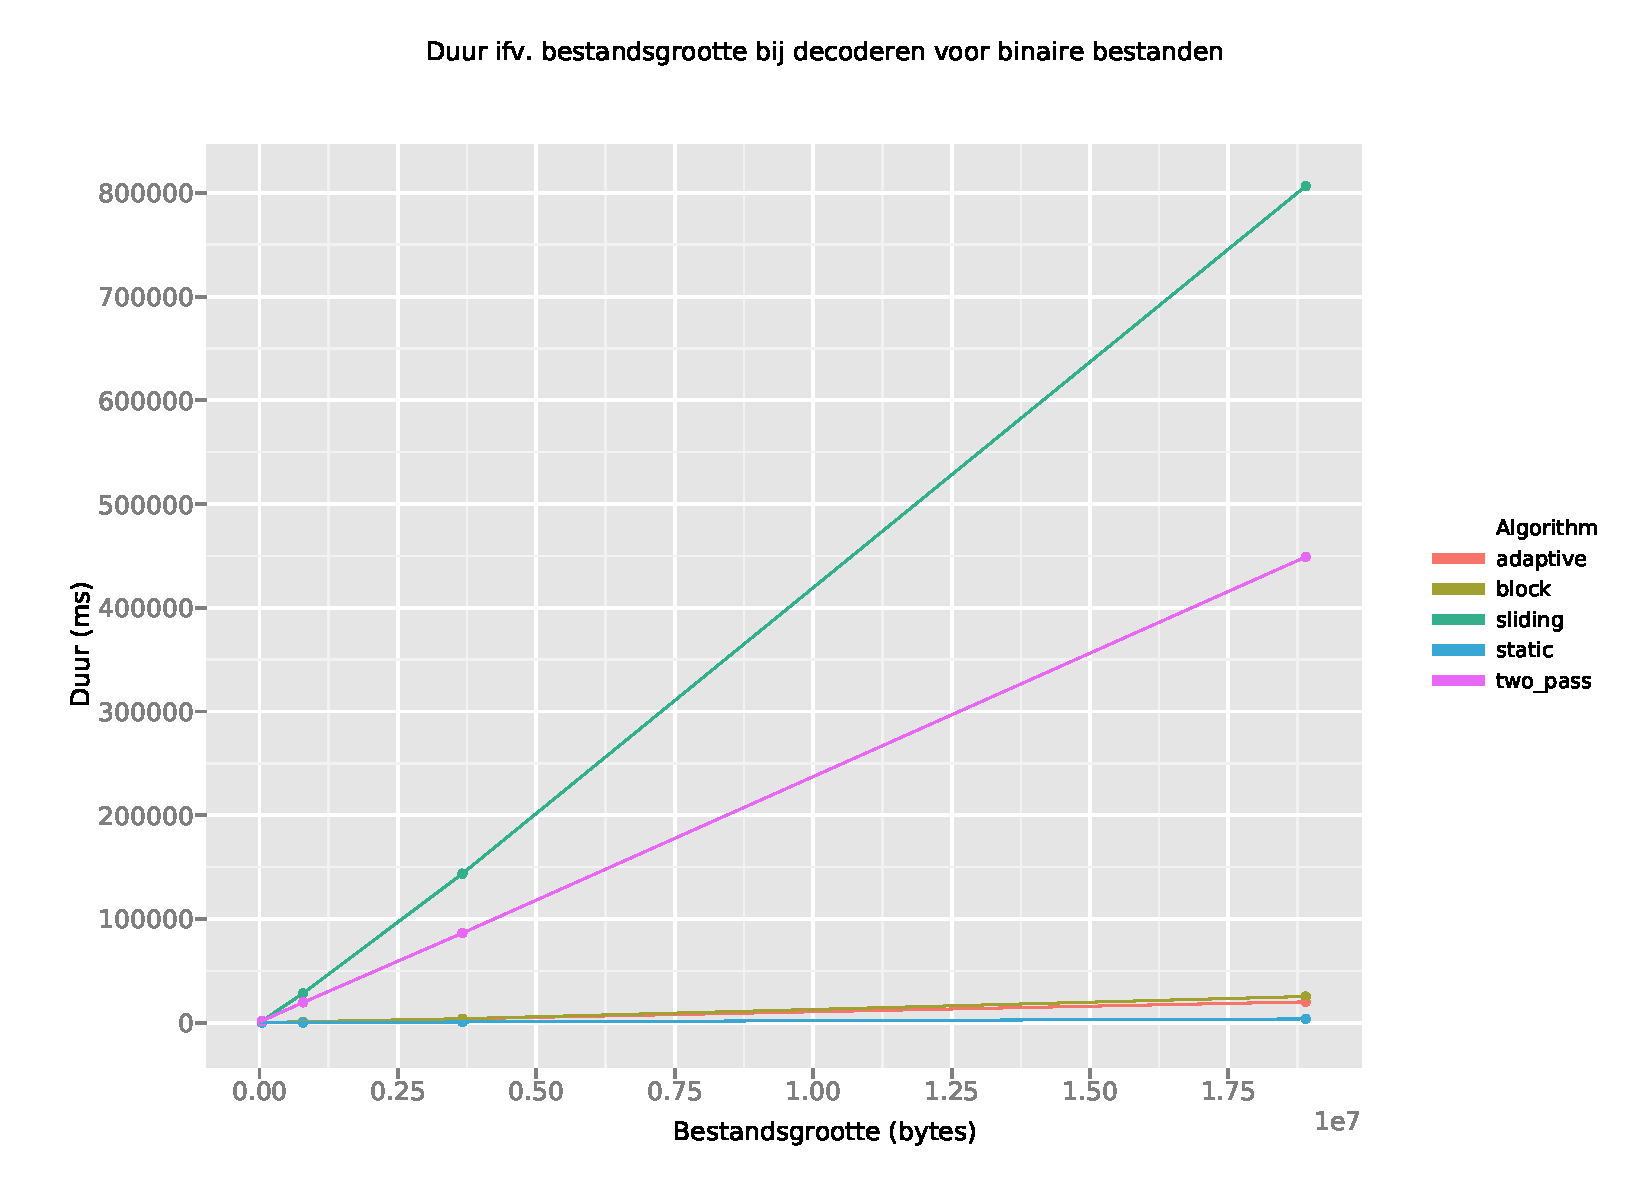
\includegraphics[width=.5\linewidth]{../experimenten/grafieken/duur/decode_binaire_bestanden.pdf}
%	\end{subfigure}
%\end{figure}

\chapter{Besluit}
%%%%%Statisch
\section{Statische huffman}

%%%%%Adaptive huffman
\section{Adaptive huffman}


%%%%%%%%Adaptive huffman met sliding window
\section{Adaptive huffman met sliding window}

%%%%%Two pass
\section{Two pass adaptive huffman}

%%%%%Blocksgewijze adaptive huffman
\section{Bloksgewijze adaptive huffman}

%%%%%Bloksgewijze adaptive huffman
\end{document}